\documentclass{revtex4-2}
\usepackage{siunitx}
\usepackage{graphicx}

\begin{document}

\title{Improving Nb\textsubscript{3}Sn Cavity Performance Using Centrifugal Barrel Polishing}
\author{Eric Viklund}
\email{ericviklund2023@u.northwestern.edu}
\affiliation{Department of Materials Science and Engineering, Northwestern University}
\affiliation{Fermi National Accelerator Laboratory}
\author{David N. Seidman}
\affiliation{Department of Materials Science and Engineering, Northwestern University}
\author{Sam Posen}
\email{sposen@fnal.gov}
\affiliation{Fermi National Accelerator Laboratory}


\date{\today}

\begin{abstract}

    Despite having superior superconducting properties, Nb\textsubscript{3}Sn SRF cavities are still impractical in many ways compared to Nb SRF cavities due to the brittle nature of Nb\textsubscript{3}Sn. One major concern is the performance degradation that can occur when a Nb\textsubscript{3}Sn experiences mechanical stresses such as during handling and tuning of the cavity. In this study we present a potential treatment for cavities that have experienced stress induced performance degradation that involves a recoating procedure. During this procedure, the degraded cavity is coated with a small amount of Sn using the vapor-diffusion method. Using this procedure we are able to recover a significant portion of the lost performance of a Nb\textsubscript{3}Sn SRF cavity.

\end{abstract}

\maketitle

\section{Introduction}
\label{sec:Introduction}

For several decades researchers have been working to implement Nb\textsubscript{3}Sn in superconducting radiofrequency (SRF) cavities. Desirable superconducting properties, such as higher superconducting transition temperature (T\textsubscript{c}) and higher superheating field (H\textsubscript{sh})\cite{liarte2017theoretical, catelani2008temperature, lin2012effect, kubo2020superfluid}, make Nb\textsubscript{3}Sn an attractive material for SRF applications. However, the material properties of Nb\textsubscript{3}Sn make it difficult to work with. The brittleness of the material introduces new challenges to the cavity manufacturing process, which must be deposited as a thin film on a bulk cavity substrate.\cite{posen2017nb3sn, pudasaini2019growth, porter2018update} The thin and brittle nature of the film makes handling and tuning of the cavity difficult due to stresses applied to the cavity. Nb\textsubscript{3}Sn cavity performance is known to degrade severly when excessive stresses are applied to the cavity. This degradation is theorized to be caused by cracks in the brittle Nb\textsubscript{3}Sn film. Cavities that suffer from degradation must be stripped and recoated with a new Nb\textsubscript{3}Sn film, which is a time consuming and expensive process.

In this study we will explore a new procedure to heal Nb\textsubscript{3}Sn cavities that have been degraded. This procedure utilizes a short Nb\textsubscript{3}Sn recoating to heal cracks that have formed in the cavity without the need to remove the original film. Using this procedure, we are able to recover a large portion of the performance of a degraded Nb\textsubscript{3}Sn cavity with just a single furnace treatment.


\section{Experiment}
\label{sec:Experiment}

The cavity was coated using high-temperature nucleation step to create a low roughness Nb\textsubscript{3}Sn film. An in-depth analysis of this cavity coating and initial performance of the cavity was published by Posen et. al.~\cite{posen2021advances}. 

After testing the performance of the cavity, the cavity was damaged during handling leading to a sharp decrease in the performance. We theorize that the degradation was caused by stresses applied to the cavity during handling, which led to the formation of cracks. This type of performance degradation has previously been observed during assembly of Nb\textsubscript{3}Sn cavities~\cite{eremeev2023preservation}, and when tuning Nb\textsubscript{3}Sn cavities at room temperature~\cite{eremeev:srf2019-mop015}. This indicates that the stresses must be carefully controlled when handling Nb\textsubscript{3}Sn cavities otherwise cracks may form in the Nb\textsubscript{3}Sn film.

In an attempt to heal the cracks causing the performance degradation, we apply a recoating procedure. During this recoating procedure, the cavity was heated to \qty{1000}{\degreeCelsius} and exposed to Sn vapor for \qty{1}{\hour}. Sn vapor was provided by \qty{0.85}{\gram} of Sn heated to \qty{1250}{\degreeCelsius}. The theory behind these parameters is that only a small amount of Sn is necessary to fill in any microscopic cracks in the film, and applying too much Sn would cause the film to become too thick. During the coating only a small portion of the Sn evaporated leaving behind a large amount of the initial Sn still in the crucible. 

\section{Result}
\label{sec:Results}

After the initial coating the cavity reached a peak accelerating field of 24~MV/m and maximum Q of \num{2e10} at \qty{4}{\kelvin}. After the cavity was damaged the performance was degraded. The cavity only reached \qty{8}{\mega\volt\per\meter}. The cavity shows a decrease in quality factor around 6 \qty{6}{\mega\volt\per\meter} before quench.

\begin{figure}[h]%
    \centering%
    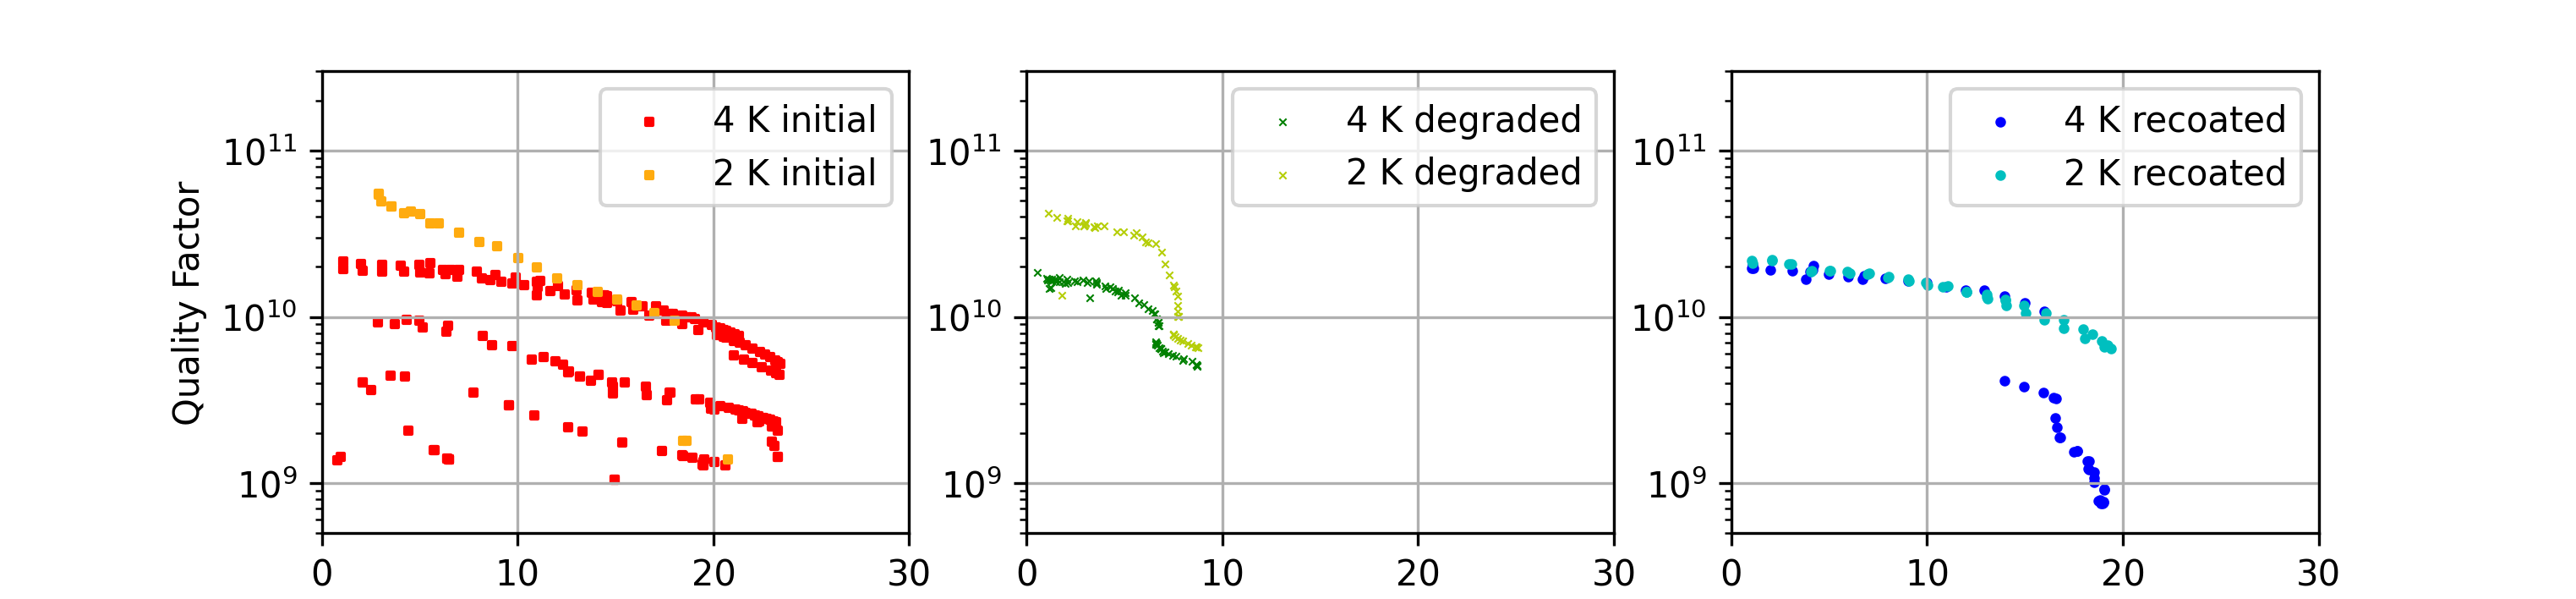
\includegraphics[width=1.0\columnwidth]{./figures/VTS.png}%
    \caption{The quality factor versus the accelerating gradient of the cavity after the initial coating (left), after the degradation (middle), and after the recoating (right).}%
    \label{fig:VTS}%
\end{figure}

\begin{figure}[h]%
    \centering%
    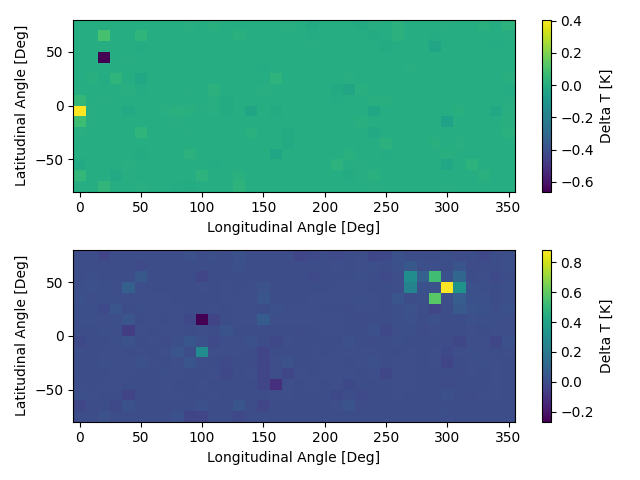
\includegraphics{./figures/TMAP.png}%
    \caption{Temperature maps of the cavity surface just before quench as measured before (top) and after (bottom) the recoating was applied.}%
    \label{fig:VTS}%
\end{figure}

Temperature mapping was used to locate the quench source responsible for the performance degradation. A single hot spot on the equator of the cavity was discovered. Visual inspection of the cavity showed no visible defects near the quench location.

After the recoating was applied the cavity performance increased. The peak accelerating gradient increased to \qty{19}{\mega\volt\per\meter} and the quality factor was \num{1e10} at \qty{4}{\kelvin}.

Temperature mapping of the cavity after the recoating shows that a similar small hotspot exists close to the equator, but the hot spot is activated at higher accelerating gradients. This indicates that the source of the degradation has been at least partially repaired by the recoating. In addition to the small hot spot near the equator, there is also a much larger hot spot closer to the iris which appears just before the cavity quench. This additional hotspot is accompanied by a large increase in x-ray production, which could indicate the heating is caused by field emission. It is possible that the cavity is limited by the multipacting, but higher accelerating gradients were not attainable even after \qty{5}{\hour} of processing.










\section{Conclusion}
\label{sec:Conclusion}

Using a low temperature, short duration Sn recoating process, we were able to heal a degraded Nb\textsubscript{3}Sn cavity that suffered damage during transportation. The recoating improved the maximum gradient of the cavity from \qty{8}{\mega\volt\per\meter} to \qty{19}{\mega\volt\per\meter}, which is close to the initial performance of the cavity of \qty{24}{\mega\volt\per\meter}. Temperature mapping measurements of the cavity show that a single defect on the equator of the cavity was responsible for the performance degradation. After the recoating this defect was partially healed leading to less heating and a higher maximum gradient.

This discovery provides a new tool that can be applied to similarly degraded cavities to recover performance. This will save time and money that would otherwise be spent by stripping the Nb\textsubscript{3}Sn coating and applying a new coating. The process could make Nb\textsubscript{3}Sn cavities more viable for real-world accelerator applications by reducing the cost of manufacturing and transportation errors.



\bibliographystyle{plain}
\bibliography{bib}

\end{document}